% !TeX spellcheck = en_GB
\documentclass[12pt,fleqn]{article}

\usepackage[english]{babel}
\usepackage{SpeedyGonzales}
\usepackage{MediocreMike}
%\usepackage{Blastoise}

\title{
    Project Plan and Evaluation:\\
    An Open Source Danish Knowledge Graph Language Model
}


\author{Søren Winkel Holm, Asger Laurits Schultz\\s183911, s183912}
\date{\today}

\pagestyle{fancy}
\fancyhf{}
\lhead{Søren Winkel Holm, Asger Laurits Schultz}
\chead{}
\rhead{Technical University of Denmark}
\lfoot{Plan for BSc. project}
\rfoot{Page \thepage{} of \pageref{LastPage}}

\graphicspath{{imgs/}}
\linespread{1.15}

\begin{document}
\maketitle

\section{Original Project Plan (Written March 12th)}
Natural Language Processing (NLP) is one of the subfields of Artificial Intelligence with the clearest practical applicability.
It is, however, also one of the most data hungry fields, resulting in a limited success in transferring methods from English to low-resource language domains such as Danish.
A possible mitigation of this limitation of statistical learning is the introduction of explicit knowledge in the modelling, which will be explored in this project.

The contextualized word representation model LUKE (Language Understanding using Knowledge Embeddings) \cite{luke} combines explicit knowledge of named entities mined from Wikipedia with deep learning in the form the Transformer architecture. \cite{transformer}
The primary goal of this bachelor project is to produce and analyze daLUKE, a Danish entity-aware model following the LUKE architecture.
The NLP subtask of Named Entity Recognition (NER) will be the main approach to examine the performance of the model.

As a part of the project, we aim to
\begin{itemize}
    \item reproduce existing Danish NER results on a number of public NER datasets and reproduce the NER results of the English LUKE
    \item pre-train a Danish LUKE-based model on the Danish Wikipedia
    \item fine-tune daLUKE on NER and compare its performance and predictions to existing NER models - particularly Danish BERT\footnote{\url{https://github.com/botxo/nordic\_bert}}
    \item optimize the performance of daLUKE, possibly by changes to data and architecture, and perform a open-source release of the pre-trained model
\end{itemize}

\subsection*{Learning Outcomes}%
\begin{enumerate}
    \item Understand and apply a Machine Learning approach that combines explicit knowledge with statistical learning
    \item Apply the training of Deep Natural Language Processing models to a low resource language
    \item Implement an open-source Deep Learning model, allowing easy reproduction and application
    \item Compare and analyze performance of Natural Language Processing models on an entity-related task and discuss their practical use
\end{enumerate}

\begin{figure}[H]
    \centering
        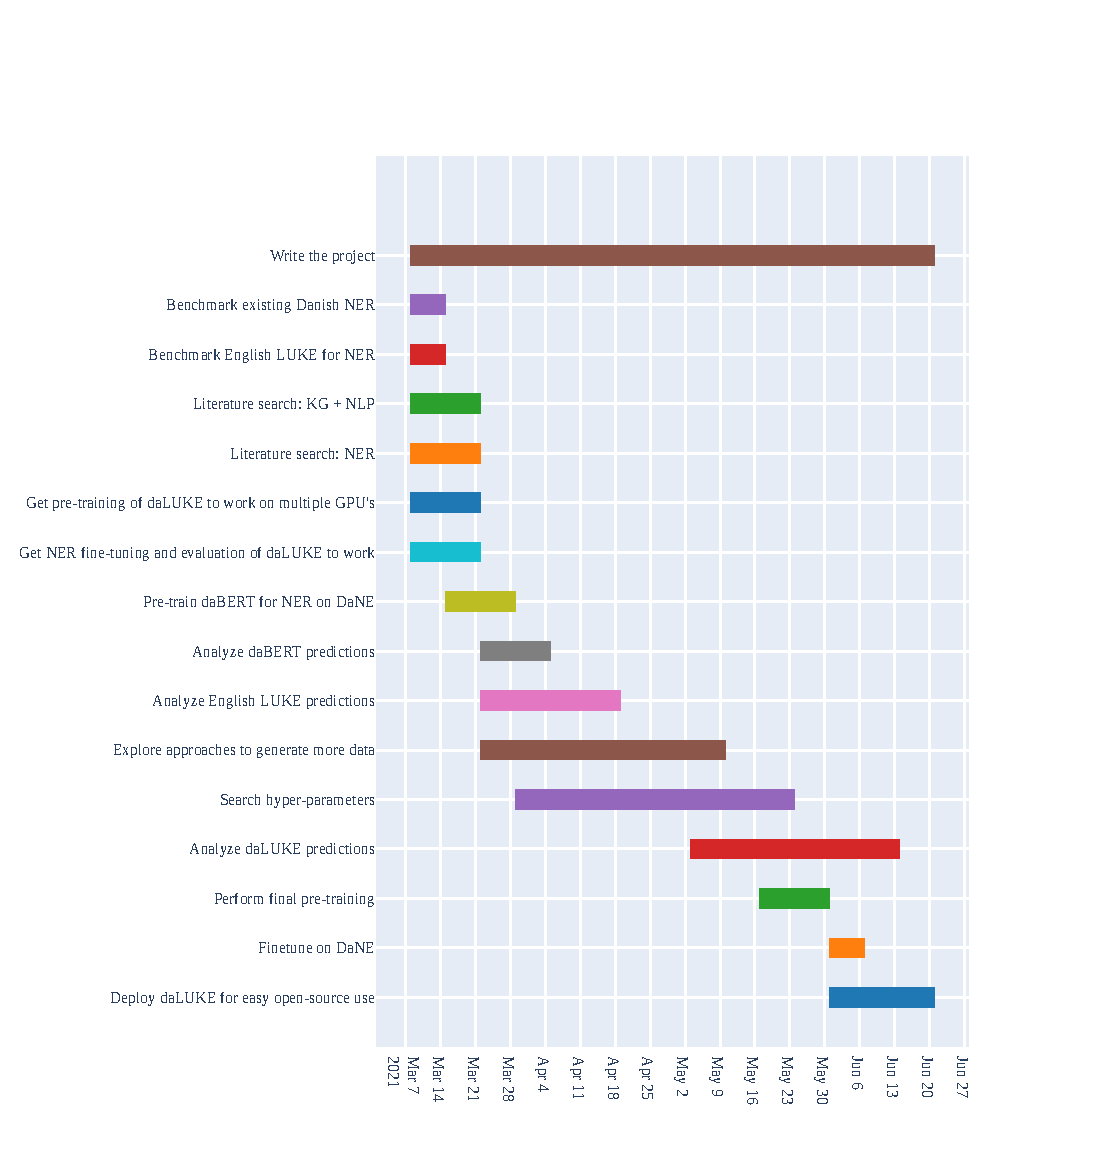
\includegraphics[width=\linewidth]{gantt}
        \caption{Gantt chart showing the current, quite tentative, project timeline}
    \label{fig:gantt}
\end{figure}\noindent

\section{Modifications and Evaluation}
The original project plan, written early in the project, has ended up not needing any significant changes regarding the goals of the project.
It lists four specific goals and four learning outcomes, all of which were successfully achieved.

However, the road was long and winded, with the original timeline on Figure \ref{fig:gantt} having little to do with reality.
At the time of the original project plan, our idea was to use the code written by Yamada et al. for LUKE and then fit it to our needs, making only minor adjustments and writing code for analysis.
This turned out to be easier said than done.
The LUKE code has next to no documentation, leaving us to guess on functionality of parts of the code based off of function names.
Furthermore, dependency handling was very challenging, and the multi GPU code straight up did not work on our cluster.
After a few weeks of battling with the code, we decided in accordance with our supervisors to rewrite the entire code base from scratch, which pushed the entire timeline by a couple of weeks, limiting how many nice-to-have analyses we would have time to make in the end.

In the end, rewriting the code turned out to be the right decision.
It gave us more control of the code, and it was a significant help in getting to understand LUKE, as we had to work with it in much closer detail than we otherwise would have.

A trap easily sprung is starting too late on the writing, requiring significant amounts of caffeine in the final days to finish the report.
As evident on Figure \ref{fig:linecounts}, we made an effort to start writing early.
This early writing primarily focused on the topic introduction, datasets and reproduction efforts.
However, by mid March, writing almost ceased completely as this was when we started rewriting the LUKE code.
When the code was ready, the model had to be trained, which would have taken about a week had it not been for the discovery of several major bugs, prompting multiple training restarts and delaying finishing the final model.
As a model was a prerequisite for making most of the experiments and analyses that we wanted to, this significantly delayed when could start writing much of the report.
We resumed writing the report in late May (see Figure \ref{fig:linecounts}), giving us about a month to write most of the report.
Despite this late start, we managed to have an early draft ready with a week to spare, letting us have a mostly stress-free end to the project with time to add nice-to-haves.

All in all, we consider the project a success.
We worked well together with no personal issues hindering work, our goals were met, and we learned a lot.
We must thank our supervisors and everyone else involved for their insight and help.
\begin{figure}[H]
    \centering
    \includegraphics[width=\textwidth]{Linecounts}
    \caption{
        Progress of the code base and report writing over time.
        Measured by counting the number of non-empty lines in Python and \LaTeX\ files every commit in the code and report repositories, respectively.
    }
    \label{fig:linecounts}
\end{figure}\noindent

\begin{thebibliography}{9}
    \bibitem{transformer} Vaswani, A. et al.: "Attention is all you need". \url{https://arxiv.org/abs/1706.03762v5}
    \bibitem{luke} Yamada, Ikuya et al. “LUKE: Deep Contextualized Entity Representations with Entity-aware Self-attention.” ArXiv abs/2010.01057 (2020)

\end{thebibliography}


\end{document}
